\documentclass[acmsmall,screen,nonacm]{acmart}
\usepackage{graphicx} % Required for inserting images

\newcommand{\todo}[1]{{\color{red} {#1}}}          % shortcut for visible remark

\title{Rewrite Rule Synthesis: A Survey}
\author{Charles Hong}
\affiliation{%
  \institution{UC Berkeley}
  \country{USA}
}
\email{charleshong@berkeley.edu} 

\date{April 29, 2024}

\begin{document}

\begin{abstract}
Rewrite rule synthesis, the automated generation of rewrite rules for program optimization and verification, presents a promising avenue for enhancing developer productivity and uncovering novel optimization strategies. However, navigating the vast space of possible rewrite rules while ensuring their correctness and effectiveness poses significant challenges. This survey explores the landscape of existing rewrite rule synthesis techniques, analyzing their strengths and limitations across three key dimensions: enumeration order, filtering mechanisms, and verification methods. We examine foundational approaches such as Knuth-Bendix completion, program synthesis-based methods employed in Halide, and e-graph-driven techniques like Ruler and Enumo. Additionally, we investigate the application of rewrite rule synthesis in domains like auto-vectorization and formal verification. While current techniques offer great value in improving performance and verifiability, as well as reducing engineering effort, these benefits can vary greatly across domains. Furthermore, scalability remains a crucial challenge that must be addressed before rewrite rule synthesis can replace manual rule-writing.
\end{abstract}

% \makeatletter
% \let\@authorsaddresses\@empty
% \makeatother
\maketitle

\section{Introduction}
Declarative techniques show great promise in program analysis and optimization. Rewrite-based techniques allow programmers to declare template rules which can be applied throughout a program in order to optimize its performance, memory consumption, or other attributes. Large optimizations can be built up from many smaller ones, applied in different orders. Declarative program optimization also allows for program optimizations to be expressed independently from program function, and such techniques have been successfully adopted in systems such as Halide~\cite{jrk2013halide}, a domain-specific language for writing high-performance image processing pipelines. Term rewriting systems have been applied to more general languages as well; for example, Haskell has long supported user-written rewrite rules in the Glasgow Haskell Compiler~\cite{peytonjones2001playing}. More recently, equality saturation and e-graphs (short for equivalence graphs) have gained significant attention, with performant implementations such as the egg library~\cite{willsey2021egg} enabling e-graphs to be used for a variety of applications, ranging from tensor graphs~\cite{yang2021tensat} to optimization of hardware arithmetic datapaths~\cite{coward2023automating}. E-graphs have even been applied to rewrite rule synthesis, as discussed later in this work. 

Ultimately, most of these applications of declarative techniques rely on the programmer to manually specify potentially beneficial rewrite rules. However, writing rewrite rules is not a trivial task. It may not be clear to the programmer whether certain rewrite rules are beneficial, or even that they do not unintentionally modify the semantics of the program or cause any cycles that would prevent the rewrite system from terminating. The programmer might in some cases not be able to think of certain rules which would have provided significant benefit.
Consequently, the idea that rewrite rules can be automatically discovered rather than hand-written is highly appealing. First, in order to reduce the developer's burden, but also to identify valuable rewrite rules that may not have been thought of ad hoc, as well as to generate rewrite rules which are provably correct. 
% Before proposing new techniques for synthesizing rewrite rules, I would like to survey the area first, understand the true value of rewrite rule synthesis, and evaluate the effectiveness of today's approaches.
% Generally speaking, rewrite rule synthesis involves enumerating rewrite rule LHS, producing a reduced RHS, and an attempt to verify the correctness and sometimes the termination of the generated rule.

Today, a variety of techniques are used to synthesize rewrite rules, but the range of potential approaches is wide, and no single accepted workflow has yet emerged. In this work, we begin by discussing what makes rewrite rule synthesis difficult, then survey existing approaches, both from an algorithmic and an infrastructure standpoint. Finally, we discuss the costs and benefits of rewrite rule synthesis and how methods for rewrite rule synthesis could be improved in future work.

\section{Challenges of Rewrite Rule Synthesis}
\label{sec:challenges}
In order to frame the rest of this survey, we now discuss some of the primary challenges associated with synthesizing rewrite rules. Some of the key dimensions along which rewrite rule synthesis techniques differ are as follows:

\begin{enumerate}
    \item \textbf{Order of enumeration---}In what order does one enumerate over the set of remaining possible expressions (on either side of a rewrite rule)? What constraints are there on the size of terms? As the size of one's grammar or terms increases, the number of possible rules also increases combinatorially, so efficient search becomes more important. This can also relate to the relative priority of rewrite rules, as some settings may be more amenable to "shortcut" rules that encapsulate large changes in one rule, whereas others might prefer smaller rules that can be combined in different ways to explore the full space of rewrites.
    \item \textbf{Filtering---}How do you filter out rewrite rules such that only interesting (e.g. useful for optimization, not redundant, etc.) ones remain in the search space?
    \item \textbf{Verification---}How do you verify that the rewrite rules you generate are correct and improve programs?
\end{enumerate}

Of course, there is no unified approach for different domains, and the optimal choice in each dimension will vary by the specific programs under consideration. The metrics that can be used to evaluate the effectiveness of these tool are less clear, and will be discussed in this survey on a per-work basis.

% Additionally, there are a number of metrics that can be used to evaluate the effectiveness of a rewrite rule synthesis technique:

% \begin{enumerate}
%     \item \textbf{Performance---}Some contexts it might be more obviously program performance, but in some contexts not, e.g. Knuth-Bendix completion where you either get a confluent and terminating TRS or you don't (binary)
%     \item \textbf{Efficiency---}
%     \item different kinds of usefulness depending on the domain
% \end{enumerate}


\section{Knuth-Bendix Completion}
Knuth-Bendix completion~\cite{knuth1970completion}, proposed in 1970 and named after Donald Knuth and Peter Bendix, is a key predecessor to rewrite rule synthesis. It is a semidecision procedure for the word problem, i.e. the problem of deciding whether two expressions are equivalent with respect to a set of rewrite relations. Given a base set of equations and a reduction order on terms, if it succeeds, it provides a confluent and terminating term rewriting system that can be used to solve the word problem for the given equational theory. However, it may also fail or not terminate. In order to consider Knuth-Bendix completion's merits as a rewrite rule synthesis technique, we can take a look at where it lies along the dimensions discussed in Section~\ref{sec:challenges}.

\begin{enumerate}
    \item \textbf{Order of enumeration---}The order of enumeration is a modifiable parameter in Knuth-Bendix completion, where the steps (Delete, Compose, Simplify, Orient, Collapse, Deduce) can be run in a user-determined order. The general strategy of utilizing known equalities to enumerate possible rewrites, as well as simplifying rewrites using other known rewrites, are both key techniques that can be seen in the other works in this survey.
    \item \textbf{Filtering---}Since Knuth-Bendix completion is based on a set of input equations, not on a grammar, the space of possible terms is much more limited than tools which attempt to enumerate all possible terms in a given grammar. Beyond this inherent constraint, when determining whether a rewrite rule is worth creating, the algorithm uses the provided reduction order on terms. This is powerful because we know that such an ordering exists, and in the algorithm, all generated rules $l \rightarrow r$ have $l>r$.
    \item \textbf{Verification---}Huet~\cite{huet1980complete} showed in 1980 that when the algorithm terminates, it defines a valid semidecision algorithm for the word problem.
\end{enumerate}

As it originates from computational mathematics, the initial examples provided for the usefulness of Knuth-Bendix completion relate mostly to group theory and not to actual programming systems. This makes it hard to evaluate the effectiveness of Knuth-Bendix completion from a programming systems perspective. However, it has had significant influence on later work whose value we will discuss more extensively.

\section{Rewrite Rule Synthesis for Program Optimization}

\subsection{Halide}
Halide~\cite{jrk2013halide}, a domain-specific language for high-performance image processing pipelines, utilizes a term rewriting system with over a thousand hand-written rewrite rules (as of the time of Newcomb et al.'s rewrite rule synthesis for Halide~\cite{newcomb2020verifyinghalide}). Newcomb et al. attempt to recreate Halide's existing rules, as well as generate new ones by applying program synthesis techniques.

\begin{figure}[htbp]
\centering
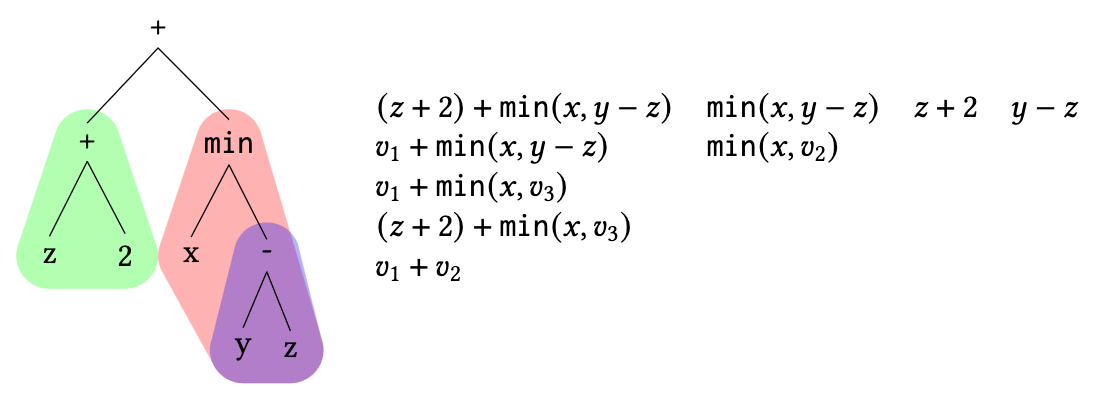
\includegraphics[scale=0.5,trim=0cm 0cm 0cm 0cm, clip]{figs/halide_bottomup.png}
\caption{Figure 3 from Newcomb et al.~\cite{newcomb2020verifyinghalide} explains how LHS patterns are mined from input expressions. In this case, $(z+2)+\texttt{min}(x,y-z)$ yields the candidate LHS terms on the right. All possible subterms are enumerated, plus copies of those terms where subterms of interest (colored in the figure) are replaced by a variable.}
\label{fig:halide_bottomup}
\end{figure}

\begin{enumerate}
    \item \textbf{Order of enumeration---}Candidate rule LHSs (left-hand sides) are enumerated and from input expression of interest, in a bottom-up order. Figure~\ref{fig:halide_bottomup} RHSs (right-hand sides) are generated via 1) “delayed” AC matching, where associativity and commutativity are applied to the LHS, and the resulting term is passed to the existing TRS, and 2) counterexample-guided inductive synthesis (CEGIS), used in sketching for program synthesis~\cite{solar2009sketching}, to superoptimize the LHS. 
    \item \textbf{Filtering---}Rules are pruned heuristically based on term size; the authors specifically state that terms must have seven or fewer leaves. They also keep a blacklist of LHSs which previously failed to generate a rule.
    \item \textbf{Verification---}The authors prove that the term rewriting system (TRS) terminates, based on a reduction order that closely matches the original TRS (eight existing rules had to be removed). They use SMT and Coq to prove that the rewrite rules are correct, i.e. preserve program semantics.
\end{enumerate}

One particularly interesting aspect of this work is its discussion of the value of rule synthesis. It mainly frames the value of rewrite rule synthesis as that of a development tool for someone building a term rewriting system. Understandably, they are unable to generate all the existing hand-written rules in Halide's already large corpus of rewrite rules. However, they are able to identify a number of bugs in the system, which previously relied on fuzz testing, as well as propose a number of rewrites that significantly improve memory utilization. The authors also provide a case study based on rewrite rules added late into Halide's development, showing that given relevant test expressions, synthesized rules are superior to hand-written ones with one exception not supported by CEGIS.

One potential downside this work is the size of the generated set of rules---around 4000, which is four times the size of the original large, hand-written ruleset. The majority of generated rewrite rules do not provide any benefit, and of those that do, they mainly improve memory usage and not runtime. This also makes the term rewriting system more difficult for both humans and verification tools to reason about, although the the authors state that the added rules had no significant impact on performance of the compiler itself.

\subsection{Ruler}
\label{sec:ruler}

\begin{figure}[htbp]
\centering
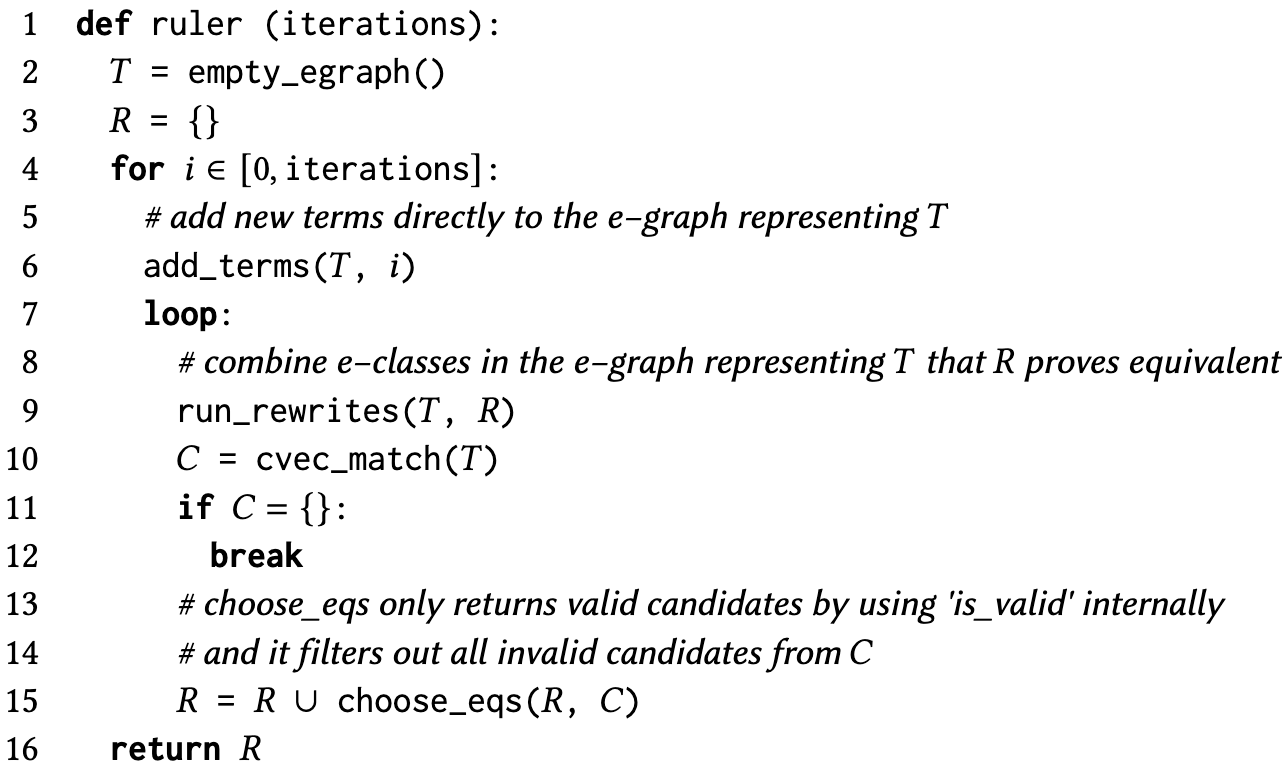
\includegraphics[scale=0.5,trim=0cm 0cm 0cm 0cm, clip]{figs/ruler_algo.png}
\caption{Figure 4 from Ruler~\cite{nandi2021ruler} shows Ruler's core algorithm. Note that at each iteration, all terms up to size $i$ are added to the e-graph (Line 6, \texttt{add\_terms()}). Equivalences between these terms are then identified via fingerprinting, and rewrite rules are extracted from newly crafted e-classes.}
\label{fig:ruler_algo}
\end{figure}

Ruler~\cite{nandi2021ruler} uses equality saturation as a rewrite system on the domain of rewrite rules itself. The authors boil rule inference down into three key steps, and demonstrate the effectiveness of their approach by implementing rule synthesis for booleans, bitvectors, and rationals. The three steps are as follows:
\begin{enumerate}
    \item \textbf{Enumerate} terms into a set $T$. Terms are enumerated from the target domain and represented in an e-graph (equality graph), a data structure for efficiently managing equivalence classes of terms. As shown in Figure~\ref{fig:ruler_algo}, at each iteration, all terms up to a specific size are added to the e-graph.
    \item Search $T \times T$ for a set of candidate equalities $C$. Pairs of potentially equivalent terms are identified within the e-graph based on their characteristic vectors (cvecs), which act as fingerprints capturing term behavior under various inputs.
    \item Choose a useful, valid subset of $C$ to add to the ruleset $R$, attempting to minimize redundancy and maximize generality. A large number of heuristics is used, including favoring more distinct variables, fewer constants, shorter larger side (between the two terms forming the candidate), shorter smaller side, and fewer distinct operators. This encapsulates the \textbf{Filtering} step of the rule synthesis process.
\end{enumerate}
In terms of performance of the rewrite rule synthesizer, the key idea is to use e-graphs and equality saturation help make these steps more efficient. Specifically, the set of terms $T$ is represented using an e-graph, which is merged iteratively using equality saturation. Rewrite rule candidates are proposed based on the current set of e-classes, valid equivalences are applied to the e-graph, and so on in a loop. However, one key drawback is that given a grammar, Ruler adds \emph{all} terms of a certain size to the e-graph at each iteration, which means the number of terms grows combinatorially with the size of the grammar. As shown in the followup work Enumo~\cite{pal2023enumo}, for grammars like that of Halide, Ruler times out after just one iteration. Nonetheless, with Herbie~\cite{panchekha2015herbie}, a tool for improving floating point accuracy whose original ruleset has 52 rules, Ruler demonstrates an ability to outperform a hand-designed ruleset.

For \textbf{Verification}, Ruler supports various validation methods for candidate rules, and the authors provide their analysis of which strategies make sense in different scenarios:

\begin{itemize}
    \item Model checking: Ideal for small domains where all possible input combinations can be exhaustively checked.

    \item SMT solving: Suitable for larger domains where symbolic reasoning is more efficient than exhaustive testing.

    \item Random testing/fuzzing: Useful for domains where formal verification is impractical or where a probabilistic guarantee of soundness is sufficient.
\end{itemize}

Ruler also seeks to provide a framework for rewrite rule synthesis that is more general than those provided in prior work. Specifically, it allows domain specification via a grammar and an interpreter. Users provide a grammar that defines the syntax of the target domain, as well as an interpreter that evaluates expressions and determines their semantics. Based on these inputs, Ruler is able to enumerate possible terms within the target domain, as well as compare terms for equivalence and validate candidate rules.

Additionally, Ruler uses characteristic vectors (Cvecs) as a generalizable method for equivalence checking. Ruler tags each term in the set of terms $T$ with a Cvec which captures its value under different input values. Cvecs act as fingerprints for a quick equivalence check between terms that does not rely on domain-specific knowledge or complex symbolic reasoning. This facilitates rule discovery in diverse domains, even those with partial operators (like division) or complex semantics.

\subsection{Enumo}
Enumo~\cite{pal2023enumo} expands on Ruler by proposing a DSL for rewrite rule synthesis tools. This DSL provides operators that allow users to "strategically guide rule inference and incrementally build rulesets" by programmatically growing and shrinking the e-graph of terms, as well as the set of rules. 

In addition to the DSL, the key technique Enumo introduces that was not present in Ruler is "fast-forwarding," where user-provided information is used to explore more deeply in a suspected good direction. This specifically modifies the \textbf{Order of enumeration} axis, while the \textbf{Filtering} and \textbf{Verification} techniques remain similar to Ruler. Specifically, rule enumeration in Enumo begins with a workload rather than a full grammar. In Enumo, "Allowed" and "forbidden" operators can be specified by the user. Forbidden operators can only be added to the e-graph via a set of "exploratory rules," also specified by the user. In the Enumo DSL, the user can design their rule synthesizer to use different subsets of rules (defined by the operators used in the rules, i.e. allowed, exploratory, or all) to grow and collapse the e-graph of terms.

\subsection{Isaria}
\begin{figure}[htbp]
\centering
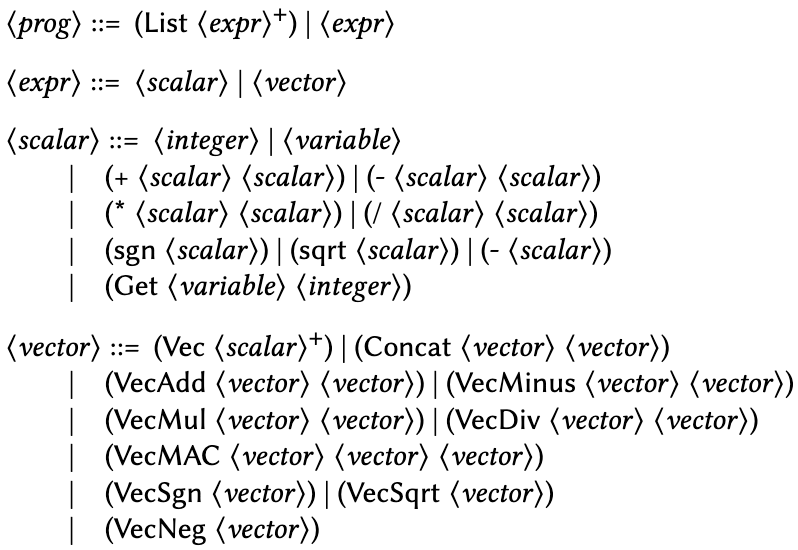
\includegraphics[scale=0.5,trim=0cm 0cm 0cm 0cm, clip]{figs/isaria_dsl.png}
\caption{Figure 1 from Isaria~\cite{thomas2024isaria}: the vector DSL used in Isaria and Diospyros~\cite{vanhattum2021diospyros}.}
\label{fig:isaria_dsl}
\end{figure}

Diospyros~\cite{vanhattum2021diospyros} utilizes e-graphs for auto-vectorization on digital signal processors (DSPs). Isaria~\cite{thomas2024isaria} rebuilds this tool, but instead of hand-writing rewrite rules, uses Ruler (with some modifications) to automatically generate them. The resulting ruleset beats Diospyros perfromance in most cases. The modifications to Ruler are as follows:
\begin{itemize}
    \item The authors add explicit support for generalizing rules for scalar computation to vectors. This prevents scalar rewrites being applied to already vectorized code, which doesn't make sense. This \textbf{Filtering} change helps stop the e-graph of terms from blowing up, which as discussed in Section~\ref{sec:ruler} is a key challenge with Ruler.
    \item Isaria automatically categorize candidate rules into 1) Expansion (roughly, scalar to scalar rewrites), 2) Compilation (scalar to vector lowering), and 3) Optimization (vector to vector rewrites) phases, based on how rules change program cost. These rules are then applied in phases during program optimization.
\end{itemize}
Again, Isaria demonstrates the scaling challenges of grammar-based rewrite rule synthesis. Despite its vector DSL being quite small (see Figure~\ref{fig:isaria_dsl}), the authors must employ domain-specific strategies that prevent all possible rewrites from being applied to the term e-graph.

\section{Rewrite Rule Synthesis for Verification}

\subsection{CVC4}
N{\"o}tzli et al.~\cite{notzli2019cvc4} build a tool that automatically generating rules to rewrite terms for Satisfiability Modulo Theories (SMT) solvers. In this case, the goal of rewrites is to pre-process input terms by simplifying them to a form that is friendly to the solver. While the objective may differ, we can still investigate where this work lies on our three axes.

\begin{enumerate}
    \item \textbf{Order of enumeration---}In this work, the authors utilize Syntax-Guided Synthesis (SyGuS)~\cite{alur2013sygus} to enumerate potential rewrite rules starting with a grammar. Enumeration starts with smaller terms and progressively explores larger ones while adhering to a specified size limit. This prioritizes "simpler" rewrite rules.

    \item \textbf{Filtering---}The user provides a SyGuS specification, which "acts as a filtering mechanism to discard terms that should not be included in rewrite rules." In addition, this work employs multiple techniques to filter out redundant or uninteresting terms, including:
    
    \begin{itemize}
        \item Matching: Eliminates terms that are instances of previously generated rewrite rules.
        \item Variable Ordering: Discards terms where variables appear in a non-canonical order, assuming a certain symmetry in the grammar.
        \item Congruence Closure: Removes terms that can be deduced from existing rules through congruence reasoning.
    \end{itemize}
        
    \item \textbf{Verification---}The paper introduces an optional mode in CVC4 that checks the soundness of the generated rewrite rules. This mode employs grammar-based sampling to find potential counterexamples where the original term and its rewritten form have different values.
\end{enumerate}

In addition, this work discusses the wide range of metrics that could be considered for the rewrite rule synthesis problem, and discusses how their workflow fares under those metrics. Specifically, the authors ask four questions:
\begin{itemize}
    \item How does the number of unique terms scale with the number of grammar terms?
    \item How do rewriters affect term redundancy and enumeration performance?
    \item What is the accuracy and performance of different equivalence checks?
    \item How many candidate rewrites do our filtering techniques eliminate?
\end{itemize}

This discussion can be found in Section 5 of the original work. Overall, the authors find that their solution performs better than existing ones in enumeration performance and equivalence checking. However, it is notable that for the larger grammars, the tools is unable to scale past 2 or 3 terms---in line with observations from previous works which enumerate terms based on a grammar (albeit with filtering).

% \subsection{CVC4SY}
% CVC4SY~\cite{reynolds2019cvc4sy} is a SyGuS solver that employs various term enumeration techniques to explore the space of rewrites.

\subsection{Theory Exploration}
Theory exploration~\cite{buchberger2000theorema, buchberger2006theorema} is an approach to generating lemmas for verification, where valid lemmas are eagerly generated rather than being guided by a proof goal or written by hand.
These lemmas can be viewed as analogous to rewrite rules, since they represent bidirectional equivalence relations used to modify expressions into a more useful state.
In fact, Enumo~\cite{pal2023enumo}, discussed above, is presented as a theory exploration tool.
Since this survey is primarily focused on program optimization, we will briefly discuss one related work; however, this is far from a comprehensive survey of theory exploration.

TheSy~\cite{singher2021thesy} introduces a \emph{symbolic} technique for theory exploration. Like in Ruler and Enumo, the authors utilize grammar-based enumeration and build an e-graph of terms. They call their technique Syntax-Guided Enumeration, or SyGuE.
Unlike these works, TheSy uses symbolic observational equivalence (SOE), where terms are equivalence-checked on symbolic inputs. Redundant conjectures are filtered out and remaining ones are verified using induction based on algebraic data structure definitions. Overall, the similarity of this work to the above, even when the objective is verification rather than optimization, is noteworthy.

\section{Conclusion and Future Directions}
\subsection{Why synthesize rewrite rules?}
The premise of being able to generate rewrite rules from scratch, without needing to provide program or rule examples, is enticing. However, one of the main challenges of rewrite rule synthesis is scaling to larger sizes of grammar and rules. Methods that generate rewrite rules directly from a grammar (Ruler and Isaria) fail to terminate once expanded beyond academic examples. 
Isaria makes this type of grammar-based rule synthesis more tractable by preventing certain rewrites from being applied based on domain characteristics of their vector DSL. Enumo tackles the problem by designing a DSL which provides the ability to restrict synthesis with user-provided information.
Newcomb et al., after working with Halide, a production-scale language, suggest that rewrite rule synthesis should be treated as a tool more as a tool to aid developer productivity, rather than a means to replace any and all rule-writing in program optimization.

Synthesizing rewrite rules has many potential benefits. As seen in this survey, the use cases range from auto-vectorization to improving floating point accuracy to formal verification. However, the actual metrics used to evaluate rewrite rule synthesis vary greatly depending on the setting, and as seen in the CVC4 work from N{\"o}tzli et al., there are a number of questions we can ask regarding just how well our rule synthesis system is working. Improvements in performance (of the resulting system), improved verifiability, and reduced engineering effort are some of the examples of how synthesizing rewrite rules might help developers of programming systems. That being said, rewrite rule synthesis might not make sense for all systems. For example, without a starting point or a good heuristic for which rewrite rules are more beneficial than others, it is difficult to search over the space of possible rewrite rules, particularly if they can be larger than one or two operators in size. In these cases, or if you just want to implement a few basic optimizations, it might make sense to hand-write your rewrite rules (or if they are simple enough, perhaps a large language model could suggest them).

% The first goal of this survey is simply to improve my personal understanding and provide a summary of the space for anyone else interested. 
% In addition, I will discuss tradeoffs associated with different potential directions for rewrite rule synthesis. For example, I will likely discuss when it is most effective to generate rules based on the grammar itself of language under consideration, or based on example programs written in that language (or to do both).

% Also, it is unclear where exactly the greatest value of rule synthesis lies.
% Depending on the domain, the assumptions and metrics at work might change.
% Different domains might require rules with more constraints and guards. There may be domains where deeply searched, many-term rules make sense, and ones where they do not. I plan to make these tradeoffs more concrete by comparing the characteristics of different domains where rewrite rule synthesis has been applied.

\subsection{What questions remain?}

Ruler and Enumo are interesting because they try to generalize the rewrite rule inference problem and develop frameworks that can apply to a range of domains. One question that has not been heavily explored in the space of rewrite rule synthesis is engineering effort. For a given domain, would it take more time to implement a rule synthesis tool for that domain, or manually write a similarly effective (and more human-interpretable) set of rewrite rules? This is a question that may be difficult to systematically evaluate, but its answer has practical value. Of course, the development of new, more generally applicable rewrite rule synthesis techniques and frameworks will change the calculus here.

We have seen that providing synthesizers with example programs and rule heuristics can help them scale. Generally speaking, these examples and heuristics are encoded by the developer of the synthesizer. Cost models for terms exist, and are currently used by rewrite rule synthesizers like Isaria, but are not necessarily used to guide enumeration and filtering during the rule synthesis process. Could cost models be used to guide the order in which rewrite rules are enumerated, and filter rewrite rules that, say, have a left-hand side which is already performance-optimized? Furthermore, are there new methods which could be used to generate example programs or rules? And how else could scaling challenges be addressed?

Generally, the implemented systems for rewrite rule synthesis replace an existing system, which already have a set of rules that can be used for comparison. It will be interesting to see whether rewriting systems of the future can be built from the ground up with rewrite rule synthesis, or if rewrite rule synthesis will primarily serve as a helpful tool for developers of such systems, as Newcomb et al. proposed. Rewrite rule synthesis is an emerging area of research, and the projects discussed in these surveys are pioneering works in the domain. While we have seen a number of impactful use cases for rewrite rule synthesis in this survey, there may be many more yet to be discovered.

\bibliographystyle{ACM-Reference-Format}
\bibliography{ref}

\end{document}
